\documentclass[12pt]{scrartcl}
\usepackage[ngerman]{babel}


\usepackage{amsmath, amssymb}

\usepackage{array}  % for the tables

\usepackage{nameref}  % for referencing with name

\usepackage{hyperref}  % for hyperlinks

\usepackage{mathrsfs}

\usepackage{graphicx}  % for the images

\usepackage{xcolor, colortbl}

\usepackage{gensymb} % for \degree

\usepackage{pgfplots}

\usepackage{tabto}

\usepackage{lipsum} % for the lipsum text

\usepackage{listings}

% Define custom colors
\definecolor{codegreen}{rgb}{0,0.6,0}
\definecolor{codegray}{rgb}{0.5,0.5,0.5}
\definecolor{codepurple}{rgb}{0.58,0,0.82}
\definecolor{backcolour}{rgb}{0.95,0.95,0.92}

% Define custom style for Python code
\lstdefinestyle{pythonstyle}{
    backgroundcolor=\color{backcolour},
    commentstyle=\color{codegreen},
    keywordstyle=\color{magenta},
    numberstyle=\tiny\color{codegray},
    stringstyle=\color{codepurple},
    basicstyle=\ttfamily\footnotesize,
    breakatwhitespace=false,
    breaklines=true,
    captionpos=b,
    keepspaces=true,
    numbers=left,
    numbersep=5pt,
    showspaces=false,
    showstringspaces=false,
    showtabs=false,
    tabsize=2
}

\lstset{style=pythonstyle}


\RedeclareSectionCommand[beforeskip=1cm]{section}
\RedeclareSectionCommand[beforeskip=0.5cm]{subsection}

\newcolumntype{P}[1]{>{\centering\arraybackslash}p{#1}}

\usetikzlibrary{arrows}

% \usepgfplotslibrary{external}

% \tikzexternalize

\definecolor{Gray}{gray}{0.85}

\setlength{\parindent}{0cm}

% hyperlinks
\hypersetup{
    colorlinks,
    citecolor=black,
    filecolor=black,
    linkcolor=black,
    urlcolor=black
}

\bibliographystyle{IEEetran}




\author{David Jäggli}

\title{Formelsammlung Krypto}



% ---------- Begin Main Document ----------- %



\begin{document}

\maketitle

\tableofcontents

\newpage
\section{Allg}


\section{Terminologie}


\renewcommand{\arraystretch}{1.5}
\begin{center}
    \begin{tabular}{ | m{12em} | m{25em} | }
        \hline
        \textbf{Kryptographie}         & Entwerfen von Krypto-Algorithmen                       \\
        \hline
        \textbf{Kryptoanalyse}         & Brechen von Krypto-Algorithmen                         \\
        \hline
        \textbf{Perfekte Sicherheit}   & Unendlich viele Ressourcen sind equivalent zu raten    \\
        \hline
        \textbf{Unkeyed Kryptographie} & Hashfunktionen                                         \\
        \hline
        \textbf{Symmetrische Krypt.}   & Beide den gleichen Schlüssel - $\mathcal{O}(n²)$       \\
        \hline
        \textbf{Asymmetrische Krypt.}  & Öffentlicher und privater Schlüssel - $\mathcal{O}(n)$ \\
        \hline
    \end{tabular}
\end{center}


\section{Symmetrische Kryptographie}

\section{Asymmetrische Kryptographie}

\newpage
\section{Blinde Signaturen}

Generelle Beschreibung: Anna weis nicht WAS sie unterschreibt, wenn sie das Dokument später sieht,
weis sie aber DASS sie es unterschrieben hat.\\
Nutzen:
\begin{itemize}
    \item Unverfällschbarkeit
    \item Anonymität
    \item Unlinkbarkeit
\end{itemize}

\vspace{0.5cm}
\noindent
Ablauf:
\label{sec:dinimam}
\begin{enumerate}
    \item Kunde zieht geld ab
    \item Bank signiert den Betrag
    \item Kunde bezahlt im Shop
    \item Shop schickt die Unterschrift an die Bank
    \item Bank prüft Unterschrift
    \item Bank validiert Unterschrift und zieht Geld ab
\end{enumerate}

\vspace{0.5cm}
Beispiel: Siehe s.100 Folien 09


\section{Einführung in die Public-Key Infrastruktur (PKI)}

\subsection{Verschlüsseln und Signieren (repetition)}

% TODO: verlinken zu initialem Kapitel

\subsubsection{Verschlüsseln}

\subsubsection{Signieren}

\textbf{Ablauf signieren:}

\begin{enumerate}
    \item Dokument von Alice ist Ausgangswert
    \item Hash berechnen $\rightarrow$ Hashwert
    \item chiffrieren (mit private key und Hash) $\rightarrow$ Signatur
    \item Dokument \& Signatur + Zertifikat $\rightarrow$ signiertes Dokument
\end{enumerate}

Warum Zertifikat? $\rightarrow$ um sicherzustellen, dass der öffentliche Schlüssel auch wirklich
von Alice ist.

\newpage
\textbf{Ablauf Signatur prüfen:}
\begin{enumerate}
    \item Dokument von Alice ist Ausgangswert
    \item Signatur mit öffentlichem Schlüssel entschlüsseln $\rightarrow$ Hashwert
    \item Hashwert von Dokument berechnen
    \item Hashes vergleichen
    \item Zertifikat Überprüfen
\end{enumerate}


\subsection{Zertifikate}

\subsubsection{Herstellung eines Zertifikats}


\begin{enumerate}
    \item Zertifikatsinhalt
          \begin{itemize}
              \item Version
              \item Serial Number
              \item Subject
              \item Public Key
          \end{itemize}
    \item Inhalt hashen
    \item Hash signieren
    \item Signitierter Hash + Zertifikatsinhalt $\rightarrow$ Zertifikat
\end{enumerate}

\subsubsection{Zertifikatsklassen}

\begin{itemize}
    \item \textbf{Klasse 1:} wenig Sicherheit, keine Identitätsprüfung
    \item \textbf{Klasse 2:} mittlere Sicherheit, schwache Identitätsprüfung
    \item \textbf{Klasse 3:} hohe Sicherheit, strenge Identitätsprüfung
    \item \textbf{Qualified Certificate:} höchste Stufe, werden nur für natürliche Personen ausgestell
\end{itemize}


\newpage
\section{Protokolle}
% TODO: missed some parts until page 22


\subsection{User Authentication}

\begin{itemize}
    \item Username / Password
    \item One-Time Password
    \item Symmetric Algorithms
    \item Public-Key Algorithms
    \item Biometric Authentication
\end{itemize}

\vspace{0.5cm}
\subsection{False-rates}
Es gibt zwei Arten von False-rates:
\begin{itemize}
    \item False Acceptance Rate (FAR)
    \item False Rejection Rate (FRR)
\end{itemize}

Beide sollten so tief wie mögliche sein. Aber es ist ein Tradeoff zwischen den beiden.
Senkt man die Eine erhöht sich die Andere.


\subsection{Verifikationen}
\subsubsection{One to many}
Handy: überprüfe ob ich derjenige bin, der ich vorzugeben behaupte.


\subsubsection{Many to one}
Bank: überprüfe ob ich derjenige bin, der ich vorzugeben behaupte.


\newpage
\subsection{Paralellsession Attacke}
Zwei Sessions eröffnen, dann muss nichts gerechnet werden und Zufalls-/Chiffrierzahl
kann kopiert werden.

\begin{figure}[ht]
    \centering
    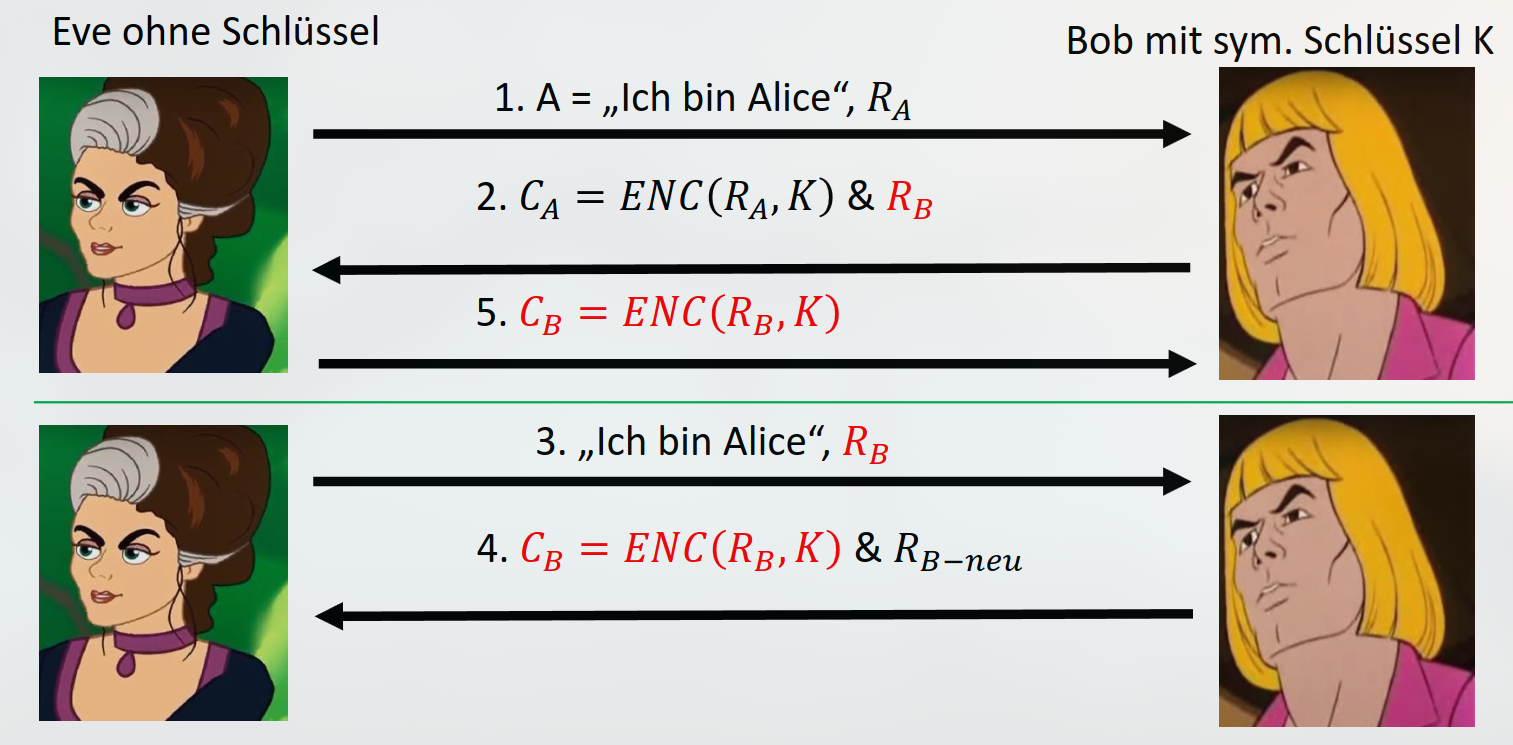
\includegraphics[width=\textwidth]{img/paralell_session_attack.png}
    \caption{Paralellsession Attacke}
    \label{fig:paralell_session_attack}
\end{figure}


\newpage
\section{Quantenkryptographie}

Quantenkryptographie und Quantencomputer sind zwei verschiedene Dinge.

\subsection{Polarization}

4 Zustände, jedem muss 1 oder 0 zugewiesen werden.

\begin{itemize}
    \item Senkrecht
    \item Wagrecht
    \item Schräg links
    \item Schräg rechts
\end{itemize}

Darauf basierend können Filter kreiert werden. Sollte filter nicht auf Teilchen
passen, ist es 50/50 in welchem Zustand es durchgelassen wird.


\subsection{Quantum Key Exchange}

\begin{enumerate}
    \item Sender Alice wählt zufällige Bits
    \item Alice sendet Photonen mit gewählter Polarization
    \item Empfänger Bob wählt zufällige Filter
    \item Bob erhlält gefilterte Photonen
    \item Bob kennt die Kodierung und ordnet 1 oder 0 zu
    \item Bob sendet zurück, welche Filter er benutzt hat
    \item Alice sagt, welche Filter korrekt waren
\end{enumerate}


Im statistischen Mittle werden in 50\% die falschen Filter gewählt. Deshalb
müssen doppelt so viele Photonen gesendet werden, wie benötigt werden. \\


Key-takeaway: immer die Bits verwenden, welche durch den Filter nicht verändert werden. Alle
anderen haben einen nicht vorhersagbaren Zustand.




% ---------- End Main Document ----------- %


% image example
% \begin{figure}[ht]
%     \centering
%     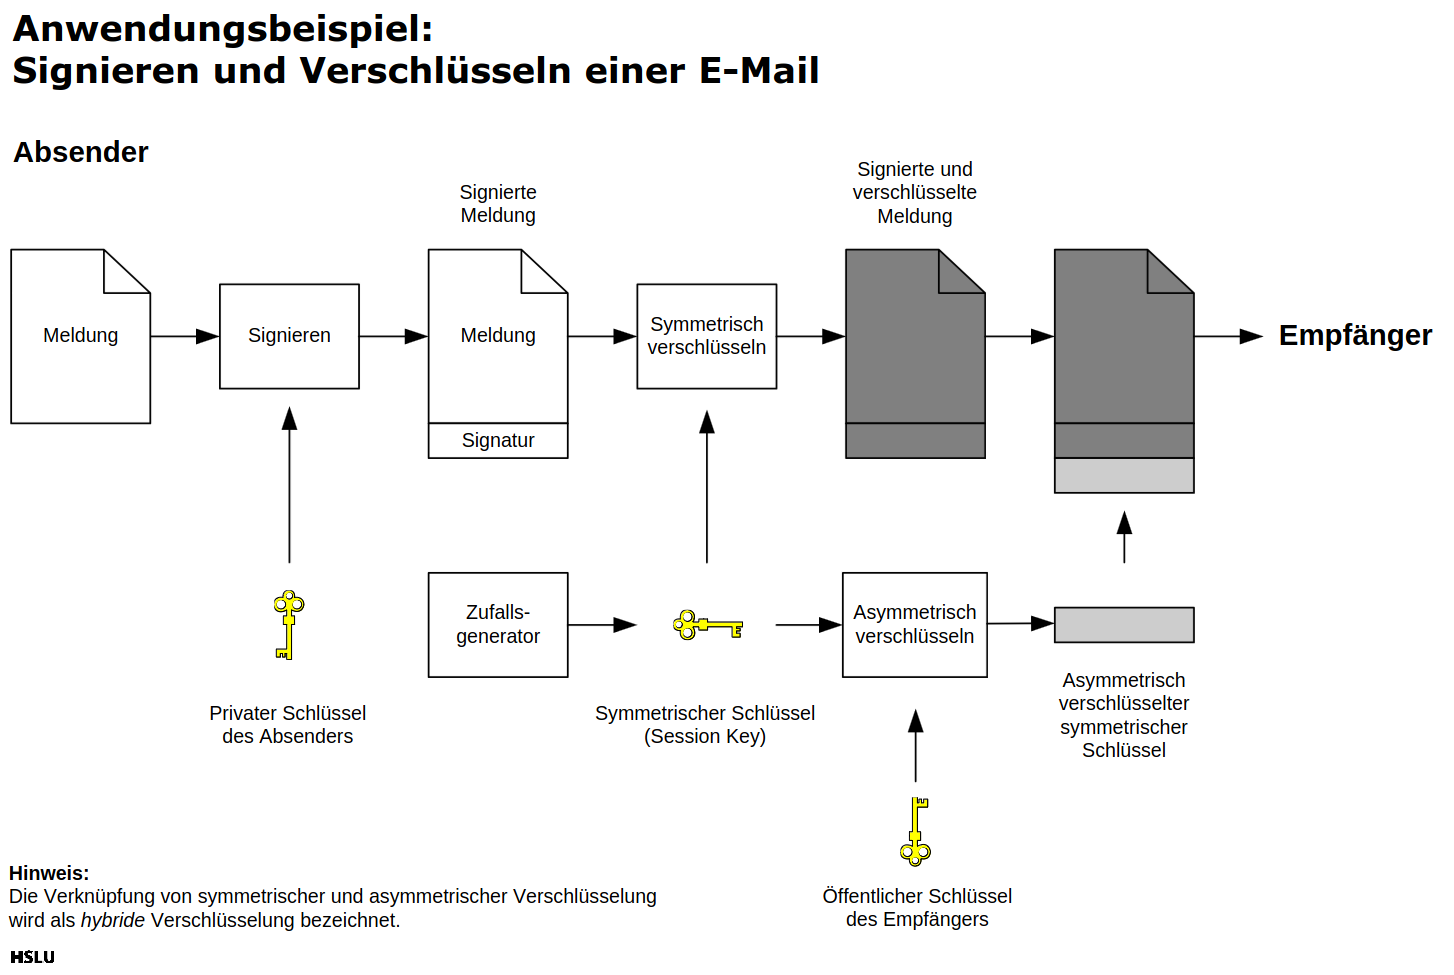
\includegraphics[width=\textwidth]{img/Anwendungsbeispiel_signieren.png}
%     \caption{Anwendungsbeispiel Signieren}
%     \label{fig:your_label}
% \end{figure}



% \begin{align*}
%     587 &= 1 \cdot 392 + 195 \\
% \end{align*}

% Matrix example
% $
% \begin{bmatrix}
%     a_{1,1} & a_{1,2} & a_{1,n}\\
%     a_{2,1} & a_{2,2} & a_{2,n}\\
%     a_{m,1} & a_{m,2} & a_{m,n}
% \end{bmatrix}$\\

% tabular example 3 columns
% \renewcommand{\arraystretch}{1.5}
% \begin{center}
%     \begin{tabular}{ | m{12em} | m{12em} | m{12em} | }
%         \hline
%         1 & 2 & 3\\
%         \hline
%         1 & 2 & 3\\
%         \hline
%         1 & 2 & 3\\
%         \hline
%     \end{tabular}
% \end{center}


% tabular example 2 columns
% \renewcommand{\arraystretch}{1.5}
% \begin{center}
%     \begin{tabular}{ | m{17em} | m{17em} | }
%         \hline
%         1 & 2\\
%         \hline
%         1 & 2\\
%         \hline
%         1 & 2\\
%         \hline
%     \end{tabular}
% \end{center}


% \begin{tikzpicture}[line cap=round,line join=round,>=triangle 45,x=0.5cm,y=0.25cm]
%     \begin{axis}[
%     x=0.75cm,y=0.5cm, % size of the grid
%     axis lines=middle,
%     ymajorgrids=true,
%     xmajorgrids=true,
%     xmin=-10,
%     xmax=10,
%     ymin=-10,
%     ymax=10,
%     xtick={-11,-10,...,10},
%     ytick={-10,-9,...,9},]
%     \draw[line width=2pt,color=blue] () -- (-2,-1);
%     \begin{scriptsize}
%         \draw[color=blue] (-9.866,-4.728) node {$g$};
%         \draw[color=blue] (-1.906,7.172) node {$f$};
%         \draw[color=blue] (3.134,5.232) node {$h$};
%     \end{scriptsize}
% \end{axis}
% \end{tikzpicture}




% \bibliography{quantum_ready}

\end{document}
